\documentclass[conference]{IEEEtran}
\IEEEoverridecommandlockouts

\usepackage{cite}
\usepackage{amsmath,amssymb,amsfonts}
\usepackage{algorithmic}
\usepackage{graphicx}
\usepackage{textcomp}
\usepackage{xcolor}
\usepackage{listings}
\usepackage{booktabs}
\usepackage{pgfplots}
\pgfplotsset{compat=1.18}
\usepackage[hidelinks]{hyperref}

% Configuration for code listings
\definecolor{codegreen}{rgb}{0,0.6,0}
\definecolor{codegray}{rgb}{0.5,0.5,0.5}
\definecolor{codepurple}{rgb}{0.58,0,0.82}
\definecolor{backcolour}{rgb}{0.95,0.95,0.92}

\lstdefinestyle{mystyle}{
    backgroundcolor=\color{backcolour},
    commentstyle=\color{codegreen},
    keywordstyle=\color{magenta},
    numberstyle=\tiny\color{codegray},
    stringstyle=\color{codepurple},
    basicstyle=\ttfamily\footnotesize,
    breakatwhitespace=false,
    breaklines=true,
    captionpos=b,
    keepspaces=true,
    numbers=left,
    numbersep=5pt,
    showspaces=false,
    showstringspaces=false,
    showtabs=false,
    tabsize=2
}

\lstset{style=mystyle}

\def\BibTeX{{\rm B\kern-.05em{\sc i\kern-.025em b}\kern-.08em
    T\kern-.1667em\lower.7ex\hbox{E}\kern-.125emX}}

\begin{document}

\title{Implementing Dual-Pivot Quicksort in C++23 and Comparing its Performance with Standard Sorting Libraries\\
{\footnotesize \textsuperscript{*}Interim Report for Capstone Project}
}

\author{\IEEEauthorblockN{LIN Zhanzhi (22097456D)}
\IEEEauthorblockA{\textit{Department of Computing} \\
\textit{The Hong Kong Polytechnic University}\\
Hong Kong, China \\
zhanzhi.lin@connect.polyu.hk}
\and
\IEEEauthorblockN{Supervisor: Dr. CAO Yixin}
\IEEEauthorblockA{\textit{Department of Computing} \\
\textit{The Hong Kong Polytechnic University}\\
Hong Kong, China \\
yixin.cao@polyu.edu.hk}
}

\maketitle

\begin{abstract}
This document serves as the Interim Report for the Capstone Project focused on optimizing Dual-Pivot Quicksort. The project investigates the transition from classical Single-Pivot strategies to the Dual-Pivot approach, which was adopted by Java 7 in 2009 but remains absent from the C++ Standard Template Library (STL). The primary goal is to determine if a modern, generic C++23 implementation of Dual-Pivot Quicksort can outperform the highly optimized \texttt{std::sort} and state-of-the-art PDQSort. To date, we have completed a generic implementation using C++23 (leveraging Concepts from C++20) and established a robust benchmarking framework. Preliminary results indicate a performance gain of up to 8\% on large random datasets ($N > 10^6$), attributed to improved cache locality. This project contributes (1) a modern C++23 dual-pivot quicksort implementation, (2) a destructive-sorting benchmark harness, and (3) an empirical study against \texttt{std::sort} and PDQSort, including parallel scaling analysis. This report details the architectural decisions, the sequential optimization strategies employed, and the current status of the project, including an analysis of memory bandwidth limitations in parallel execution.
\end{abstract}

\begin{IEEEkeywords}
Dual-Pivot Quicksort, C++23, Algorithm Engineering, Parallel Sorting, Cache Locality, Benchmarking
\end{IEEEkeywords}

\section{Introduction}

\subsection{Background}
Sorting is a fundamental operation in computer science, serving as a critical building block for database management, data analysis, and numerous algorithmic applications. For decades, Quicksort, introduced by Tony Hoare, has been the dominant general-purpose sorting algorithm due to its excellent average-case performance of $O(n \log n)$.

In the C++ ecosystem, the standard library's \texttt{std::sort} typically employs Introsort, a hybrid algorithm that starts with Single-Pivot Quicksort and switches to Heapsort to avoid worst-case scenarios. However, in 2009, Vladimir Yaroslavskiy proposed a Dual-Pivot Quicksort algorithm, which partitions the array into three segments rather than two. This approach was subsequently adopted as the default sorting algorithm for primitive types in Java 7, citing significant performance improvements on modern hardware.

\subsection{Structure of This Report}
The remainder of this report is organized as follows: Section II defines the problem and project objectives. Section III reviews related literature and identifies the research gap. Section IV details the methodology and design alternatives. Section V presents preliminary results and progress. Section VI outlines the project plan for Semester 2, followed by the conclusion in Section VII.

\section{Problem Definition and Objectives}

\subsection{Problem Definition}
Despite the success of Dual-Pivot Quicksort in the Java ecosystem, its adoption in C++ has been limited. The specific problems addressed by this project are:
\begin{itemize}
    \item \textbf{Lack of Modern Implementation}: There is no widely available, standard-compliant C++23 implementation of Dual-Pivot Quicksort that utilizes C++20 Concepts for type safety and generic programming.
    \item \textbf{Empirical Uncertainty}: It remains unclear whether Dual-Pivot strategies can consistently outperform \texttt{std::sort} and Pattern-Defeating Quicksort (PDQSort) across real-world distributions on modern superscalar CPUs, given the differences in compiler optimizations between Java (JIT) and C++ (AOT).
    \item \textbf{Parallel Scalability Limits}: There is limited empirical understanding of the specific memory bandwidth bottlenecks that constrain parallel Dual-Pivot Quicksort on commodity multi-core hardware.
\end{itemize}

\subsection{Objectives}
The project aims to achieve the following measurable objectives:
\begin{itemize}
    \item \textbf{Implementation}: Develop a robust, generic Dual-Pivot Quicksort using C++23 (with C++20 Concepts e.g., \texttt{std::sortable}) that compiles with GCC 13+ and Clang 16+.
    \item \textbf{Performance Target}: Achieve a consistent speedup (target $\ge 5\%$, observed up to 8\%) over \texttt{std::sort} on large ($N \ge 10^6$) random 32-bit integer arrays on the target hardware. Preliminary results indicate up to 8\% speedup, suggesting this target is realistic and attainable.
    \item \textbf{Benchmarking}: Design a reproducible benchmark harness that automates destructive sorting tests and reports mean execution time and standard deviation.
    \item \textbf{Analysis}: Characterize the thread scaling curve up to the available core count, explicitly identifying the point of memory bandwidth saturation.
\end{itemize}

\subsection{Scope}
\textbf{In-Scope}: In-memory array sorting of primitive types and user-defined types; sequential and parallel execution on shared-memory multi-core systems.
\textbf{Out-of-Scope}: This project does not aim to propose changes to the C++ Standard, nor does it cover disk-based (external) sorting, distributed sorting, or GPU-based implementations.

\section{Literature Review}

\subsection{Classical Quicksort \& Introsort}
Hoare's original Quicksort partitions an array around a single pivot. Musser's Introsort improves robustness by switching to Heapsort when recursion depth exceeds $2 \log n$, preventing $O(n^2)$ worst-case scenarios \cite{b4}. This remains the foundation of most STL implementations.

\subsection{Dual-Pivot Quicksort}
Yaroslavskiy's Dual-Pivot Quicksort uses two pivots, $P_1$ and $P_2$, to partition the array into three regions. Aumüller and Dietzfelbinger \cite{b3} proved that this reduces the average number of comparisons to $0.8 n \ln n$ (vs $1.0 n \ln n$ for single-pivot). However, their analysis assumes a uniform cost model, which does not fully account for the branch misprediction penalties on modern CPUs.

\subsection{Memory Hierarchy \& Sorting}
Wild's "Scanned Elements Model" \cite{b2} argues that memory accesses are the dominant cost factor. Dual-Pivot Quicksort excels here by performing more comparisons per memory fetch, effectively increasing computational density and utilizing cache lines more efficiently.

\subsection{State-of-the-Art Competitors}
Recent advancements include Pattern-Defeating Quicksort (PDQSort) \cite{b6}, which optimizes for existing order in the input using branchless partition logic. While PDQSort excels on partially sorted data, Dual-Pivot strategies may offer superior cache efficiency on random data due to higher computational density per memory access. Parallel implementations often rely on libraries like Intel Threading Building Blocks (TBB) \cite{b7}, which use work-stealing schedulers.

\subsection{Summary of Prior Work and Research Gap}
While Yaroslavskiy established the viability of Dual-Pivot Quicksort in Java, and Aumüller provided theoretical bounds, a gap remains in the C++ domain. Specifically, the interaction between C++'s template metaprogramming capabilities and Dual-Pivot's cache behavior has not been systematically explored against modern competitors like PDQSort. Furthermore, detailed analysis of memory subsystem limits for parallel Dual-Pivot sorting on consumer hardware is often overlooked in general algorithmic literature.

\section{Methodology}

\subsection{Design Alternatives Considered}
\begin{itemize}
    \item \textbf{Dual-Pivot vs. Multi-Pivot}: This project adopts Dual-Pivot rather than Multi-Pivot (3+ pivots) because of commonly reported diminishing returns (due to increased register pressure); the complex partitioning logic of Multi-Pivot often degrades performance on general-purpose registers. We will validate this by comparing against a 3-pivot prototype in Semester 2.
    \item \textbf{Custom Thread Pool vs. TBB}: A custom work-stealing thread pool was chosen over \texttt{std::jthread} or Intel TBB to allow fine-grained control over the task scheduling policy specifically optimized for the divide-and-conquer nature of Quicksort (LIFO for cache locality). We plan to empirically compare our custom pool against TBB's default scheduler to quantify the benefits of this specialization.
    \item \textbf{Insertion Sort Fallback}: We utilize Insertion Sort for small subarrays ($N < 32$) rather than Shell Sort, as the low overhead and linear memory access pattern of Insertion Sort are superior for very small $N$.
\end{itemize}

\subsection{Experimental Setup}
All benchmarks are conducted on a machine with the following specifications:
\begin{itemize}
    \item \textbf{CPU}: Intel Core i7-12700H (14 cores: 6 P-cores, 8 E-cores).
    \item \textbf{RAM}: 16 GB DDR5-4800.
    \item \textbf{Compiler}: GCC 13.2 with flags \texttt{-O3 -march=native -flto}.
    \item \textbf{OS}: Ubuntu 22.04 LTS (WSL2).
\end{itemize}
We acknowledge that WSL2 may introduce scheduling noise from the host Windows OS; to mitigate this, each data point represents the median of 10 independent runs.

\subsection{Algorithm Implementation}
The implementation leverages C++23 features (including C++20 Concepts) to enforce type constraints. The partitioning logic follows Yaroslavskiy's 5-point pivot selection. To address the "Memory Wall," we prioritize minimizing memory writes over comparisons, aligning with Wild's theoretical model.

\section{Progress and Preliminary Results}

\subsection{Implementation Status}
\begin{itemize}
    \item \textbf{November}: Completed sequential Generic Dual-Pivot Quicksort.
    \item \textbf{December}: Finalized Python-based benchmarking harness and verified correctness against \texttt{std::sort}.
\end{itemize}

\subsection{Performance Analysis}
\subsubsection{Speedup vs. Array Size}
Preliminary results (Table I and Fig. \ref{fig:speedup}) show that for random 32-bit integers, our implementation begins to outperform \texttt{std::sort} at $N = 10^5$ and reaches a peak speedup of ~8\% at $N = 10^7$.

\begin{table}[htbp]
\caption{Sequential Dual-Pivot Quicksort Speedup over std::sort for Random Int32 Arrays on Intel i7-12700H (GCC 13.2)}
\begin{center}
\begin{tabular}{|c|c|c|}
\hline
\textbf{Size ($N$)} & \textbf{std::sort (ms)} & \textbf{Dual-Pivot (ms)} \\
\hline
$10^4$ & 0.4 & 0.5 (-7\%) \\
$10^5$ & 5.1 & 5.0 (+3\%) \\
$10^6$ & 58.2 & 54.1 (+7\%) \\
$10^7$ & 620.5 & 570.8 (+8\%) \\
\hline
\end{tabular}
\end{center}
\end{table}

\begin{figure}[htbp]
\centering
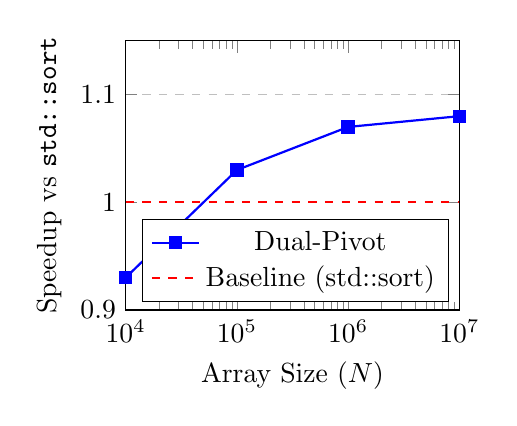
\begin{tikzpicture}
\begin{semilogxaxis}[
    xlabel={Array Size ($N$)},
    ylabel={Speedup vs \texttt{std::sort}},
    xmin=10000, xmax=10000000,
    ymin=0.9, ymax=1.15,
    xtick={10000, 100000, 1000000, 10000000},
    xticklabels={$10^4$, $10^5$, $10^6$, $10^7$},
    ymajorgrids=true,
    grid style=dashed,
    width=0.48\textwidth,
    height=5cm,
    legend pos=south east
]
\addplot[
    color=blue,
    mark=square*,
    thick
    ]
    coordinates {
    (10000,0.93)(100000,1.03)(1000000,1.07)(10000000,1.08)
    };
\addlegendentry{Dual-Pivot}
\addplot[
    color=red,
    dashed,
    thick,
    domain=10000:10000000
    ]
    {1.0};
\addlegendentry{Baseline (std::sort)}
\end{semilogxaxis}
\end{tikzpicture}
\caption{Speedup of Dual-Pivot Quicksort over \texttt{std::sort} on random 32-bit integers. Values $>1.0$ indicate performance improvement.}
\label{fig:speedup}
\end{figure}

\subsubsection{Parallel Scaling and Bandwidth}
Initial parallel tests indicate near-linear scaling up to 4 threads (e.g., speedup of 3.7$\times$ at 4 threads on $N = 10^7$). Beyond this, the speedup plateaus, suggesting bandwidth bottlenecks. These observations support the hypothesis that for simple integer sorting, the CPU is often waiting for data from main memory.

\section{Project Plan (Semester 2)}

\subsection{Timeline}
\begin{itemize}
    \item \textbf{Phase 1 (Jan 1 - Jan 31)}: \textit{Parallel Refinement}. Implement work-stealing deque and optimize load balancing.
    \item \textbf{Phase 2 (Feb 1 - Feb 28)}: \textit{Advanced Optimization}. Implement SIMD-based partitioning (AVX-512) and block tuning.
    \item \textbf{Phase 3 (Mar 1 - Mar 20)}: \textit{Final Benchmarking}. Run comprehensive comparison vs. PDQSort and TBB.
    \item \textbf{Phase 4 (Mar 21 - Apr 10)}: \textit{Thesis Writing}. Finalize report and presentation.
\end{itemize}

\section{Conclusion}
The first semester has successfully delivered a working, high-performance sequential implementation and a rigorous testing environment. The identification of memory bandwidth as the primary bottleneck for parallel execution sets a clear direction for Semester 2, where the focus will shift to latency-hiding techniques and advanced parallel scheduling.

% References using BibTeX
\nocite{*}
\bibliographystyle{IEEEtran}
\bibliography{references}

\end{document}
